  \documentclass[final]{beamer} % beamer 3.10: do NOT use option hyperref={pdfpagelabels=false} !
  %\documentclass[final,hyperref={pdfpagelabels=false}]{beamer} % beamer 3.07: get rid of beamer warnings
  \mode<presentation> {  %% check http://www-i6.informatik.rwth-aachen.de/~dreuw/latexbeamerposter.php for examples
    \usetheme{Berlin}    %% you should define your own theme e.g. for big headlines using your own logos 
   \setbeamercovered{transparent}
  }
  \usepackage[english]{babel}
  \usepackage[latin1]{inputenc}
  \usepackage{amsmath,amsthm, amssymb, latexsym}
\usepackage{tikz}
\usetikzlibrary{arrows}
\usepackage{pgfplots}
\usepackage{fix-cm}
  %\usepackage{times}\usefonttheme{professionalfonts}  % times is obsolete
  \usefonttheme[onlymath]{serif}
  \boldmath
  %\usepackage[orientation=portrait,size=a0,scale=1.4,debug]{beamerposter}                       % e.g. for DIN-A0 poster
  %\usepackage[orientation=portrait,size=a1,scale=1.4,grid,debug]{beamerposter}                  % e.g. for DIN-A1 poster, with optional grid and debug output
  \usepackage[size=custom,width=200,height=160,scale=1.4,debug]{beamerposter}                     % e.g. for custom size poster
  %\usepackage[orientation=portrait,size=a0,scale=1.0,printer=rwth-glossy-uv.df]{beamerposter}   % e.g. for DIN-A0 poster with rwth-glossy-uv printer check
  % ...
  %
  \title[]{{\fontsize{240}{240}\selectfont Title}}
  \author[]{Jialin Song and Jonathan Zung}
  \institute[University of Toronto]{Computational Biology Lab, University of Toronto}
  \begin{document}
  \begin{frame}{}
  \maketitle
    \begin{columns}[T]
      \begin{column}{0.3\linewidth}
    \begin{block}{\Huge Introduction}
    \Large
    Rare genetic disorders are caused by abnormalities in the human genome. Due to different levels of gene expressions and influences from the environment, even patients with the same underlying disorder may exhibit varying symptoms, which is a challenge for accurate diagnosis. However, clustering multiple patients with similar symptoms and utilizing the structural information in ontologies, we can uncover more information from patients.
   \vspace{3cm}

    \end{block}
    
    \begin{block}{\Huge Motivation}
    \begin{columns}[T]
      \begin{column}{.5\textwidth}
   \centering
  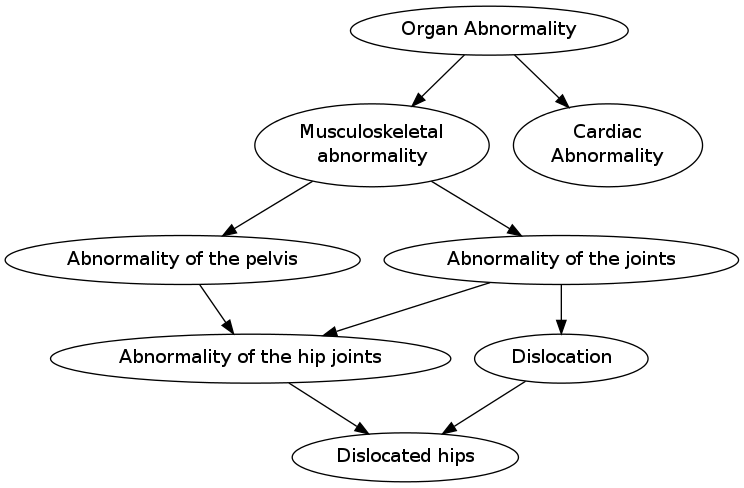
\includegraphics[width = \textwidth, height=40cm ]{hpo}
      \end{column}
      
      \begin{column}{.5\textwidth}
	    \Large
        \begin{itemize}
          \item
          HPO (Human Phenotype Ontology) provides structural information about phenotypes
          \vspace{2cm}
          \item
          OMIM (Online Mendelian Inheritance in Man) annotates disorders with HPO terms
          \vspace{2cm}
          \item
          PhenoTIps collects patients' phenotype data with standard HPO terms
          \vspace{2cm}
          \item 
          These resources enable us to develop more informed algorithms to analyse patients
      \end{itemize}  
      \vspace{5cm}
      \end{column}
    \end{columns}

    \end{block}
    \begin{block}{\Huge Objective}
     \begin{itemize}
    \Large
     \item
     Cluster patients with similar phenotypes
    \item
    Perform diagnoses on patients
     \end{itemize}
      \end{block}
    \end{column}

    \begin{column}{0.3\linewidth}
     \begin{block}{\Huge Clustering Methods}
     \Large
		\begin{block}{\Large Patient-Patient similarity metrics}
			Define a patient-patient similarity metric, and then apply a standard clustering algorithm (e.g. spectral clustering).

			Examples of similarity metrics:
			\begin{itemize}
				\item Euclidean Metric: Count number of shared traits between two patients.
				\item Information Metric: Essentially, count shared traits weighted by their rarities. Patients sharing rarer traits are more similar.
			\end{itemize}
		\end{block}
		\begin{block}{\Large Mixture Models}
			Formulate a probabilistic model for patient traits with a single latent variable $d$ representing the underlying disorder. Use the EM algorithm to fit the model, then cluster by the inferred values of the latent variable.

			Examples of mixture models:
			\begin{itemize}
				\item Independent Mixture: Traits are independent given $d$.
				\item Conditional Mixture: Traits are independent given $d$ and their ancestors in HPO.
			\end{itemize}
		\end{block}
     \end{block}
     \vspace{3cm}

     \begin{block}{\Huge Diagnosis Methods}
   
     \begin{block}{\Large Naive Bayes}
     \begin{itemize}
        \Large
    \item
    For a patient $p$, we want to find the disease $d$ with the highest conditional probability $Prob(d \mid p )$
  \vspace{1cm}
  \item
   By Bayes' Theorem: \\
   $Prob(d \mid p) = \frac{Prob(p \mid d) \times Prob(d)}{Prob(p)} \propto Prob(p \mid d) \times Prob(d)$
  \vspace{1cm}
   \item
   Naive Bayes assumes that each phenotype is independent once a disease is given \\
   $Prob(d \mid p) \propto Prob(d) \times \prod Prob(phenotype_i \mid d)$
     \end{itemize}
   \end{block}
    \vspace{3cm}

    \begin{block}{\Large Phenotype Matching}
     \begin{itemize}
     \Large
     \item
     The objective is to measure how close a patient is to the canonical form of a disorder
     \vspace{1cm}
     \item
     For each phenotype of a patient, compute the closest distances to each phenotype annotations of a disease. Construct a distance matrix from the calculated data
     \vspace{1cm}
    \item
    Use the cost matrix to determine the matching between patient's phenotypes and disease annotations that minimizes the total distance
     \vspace{1cm}
    \item
    The minimized distance representing transforming from the real patient to the canonical form of a disorder is used as the measure for closeness
         \end{itemize}
   \begin{center}
   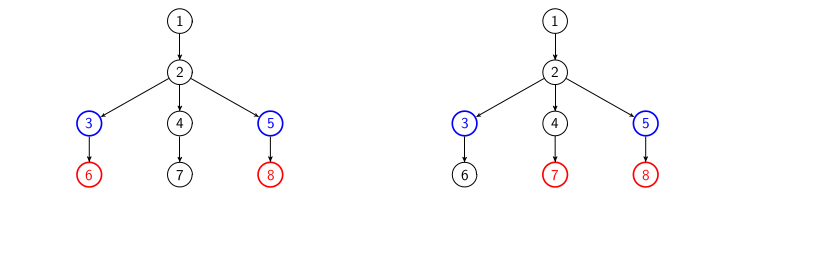
\includegraphics[width=.9\textwidth]{toy_ontology}
   \\
   \normalsize
   Figure 1: A Toy Ontology Example
   \end{center}
   \begin{columns}[T]
   \begin{column}{.9\textwidth}
   \large
Blue circles are one patient's phenotypes and red ones are annotations of a disorder. In the left one, the real patient can transform into the canonical form of a disorder via $3 \rightarrow 2 \rightarrow 4 \rightarrow 7$ and $5 \rightarrow 8$, resulting in a total cost of 4. While the right one can achieve a total cost of 2 by $3 \rightarrow 6$ and $5 \rightarrow 8$.
   \end{column}
   \end{columns}
   
   \end{block}
  \end{block}

    \end{column}

    \begin{column}{0.3\linewidth}
    \begin{block}{\Huge Results}
    \begin{block}{\Large Clustering Results }
      \centering
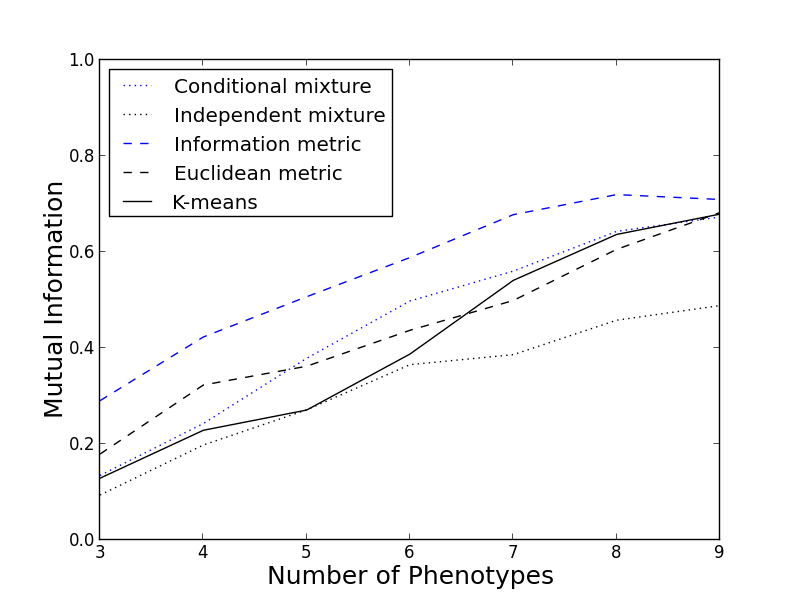
\includegraphics[width=0.7\textwidth]{cluster_comparison.png} \\
   Figure 2: Comparison of Clustering Methods

    \end{block}

    \begin{block}{\Large Diagnosis Results}

\centering
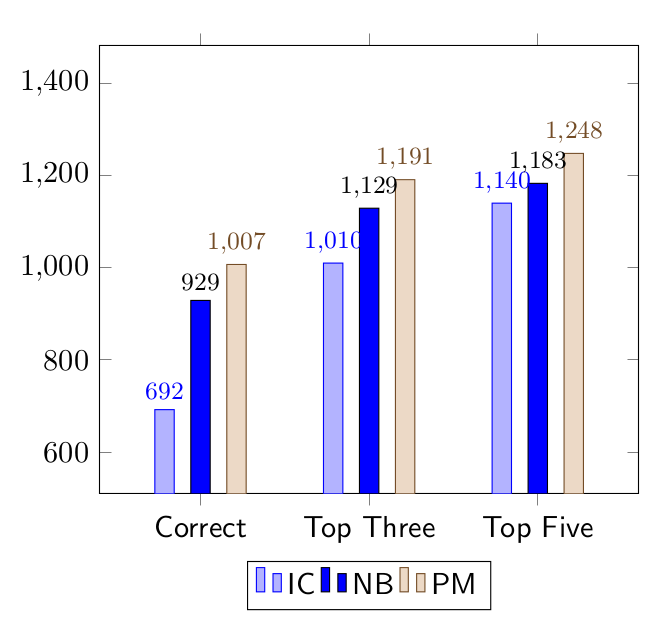
\includegraphics[width=.7\textwidth ]{sim_patients}
   \\
   Figure 3: Diagnosis Results for 1498 Simulated Patients
      \end{block}
    \end{block}
    \end{column}
    \end{columns}
  \end{frame}
  \end{document}
